\chapter{Statistics and Sampling Distributions}

\section{Statistics and Their Distributions}

Any sample mean can be regarded as a \textit{point estimate} of the population mean $\mu$.

\begin{definition}
    A \textbf{statistic} is any quantity whose value can be calculated from sample data. Prior to obtaining data, there is uncertainty as to what value of any particular statistic will result. Therefore, a statistic is a random variable and will be denoted by an uppercase letterl; a lowercase letter is used to represent the calculated or observed value of the statistic.
\end{definition}

\subsection{Random Samples}

\begin{definition}
    The rv's $X_1,\dots,X_n$ are said to form a (simple) \textbf{random sample} of size \textit{n} if 

    \begin{enumerate}
        \item The $X_i$'s are independent rv's.
        \item Every $X_i$ has the same probability distribution.
    \end{enumerate}

    Thus, $X_i$'s are \textbf{independent and identically distributed}(idd).

    The conditions are satisfied if sampling are with replacement, from an infinite population, or without replacement yet the sample size $n$ and population size $N$ satisfies $n/N\leq .05$(at most 5\% of the population is sampled).
\end{definition}

\section{The Distribution of the Sample Mean}

\begin{proposition}
    Let $X_1,\dots,X_n$ be a random sample from a distribution with mean value $\mu$ and standard deviation $\sigma$, then 

    \begin{enumerate}
        \item $E(\bar{X}) = \mu_{\bar{X}} = \mu$
        \item $V(\bar{X}) = \sigma_{\bar{X}}^2 = \sigma^2/n$ and $\sigma_{\bar{X}} = \sigma / \sqrt{n}$
        \item $E(T_o) = n\mu$
        \item $V(T_o) = n\sigma^2$ and $\sigma_{T_o} = \sqrt{n}\sigma$
    \end{enumerate}

    where $T_o = X_1 + \cdots + X_n$.
\end{proposition}

\subsection{The Case of a Normal Population Distribution}

\begin{proposition}
    Let $X_1,\dots,X_n$ be a random sample from a normal distribution with mean $\mu$ and stardard deviation $\sigma$. Then for any $n$, $\bar{X}$ is normally distributed(with mean $\mu$ and standard deviation $\sigma/\sqrt{n}$), as is $T_o$(with mean $n\mu$ and standard deviation $\sqrt{n}\sigma$).
\end{proposition}

\subsection{The Central Limit Theorem}

\begin{theorem}{THE CENTRAL LIMIT THEOREM(CLT)}
    Let $X_1,\dots,X_n$ be a random sample from a distribution with mean $\mu$ and variance $\sigma^2$. Then, in the limit as $n\rightarrow\infty$, the standardized versions of $\bar{X}$ and $T_o$ have the standard normal distribution. That is, 

    \begin{align*}
        \lim_{n\rightarrow\infty}P\left(\frac{\bar{X}-\mu}{\sigma/\sqrt{n}}\leq z\right) = P(Z\leq z)=\Phi(z) \\
    \end{align*}
    
    and 
    
    \begin{align*}
        \lim_{n\rightarrow\infty}P\left(\frac{T_o-n\mu}{\sqrt{n}\sigma/\sqrt{n}}\leq z\right) = P(Z\leq z)=\Phi(z) \\
    \end{align*}

    where $Z$ is a standard normal rv. $\bar{X}$ and $T_o$ are \textbf{asymptotically normal}.
\end{theorem}

Practical use of CLT: when $n$ is large and we wish to calculate a probability such as $P(a\leq \bar{X}\leq b)$, we need only to pretend that $\bar{X}$ is normal, standardize it and use the normal table. The resulting answer will be approximatedly correct, as shown in Figure \ref{fig:6-1}.

If $n>30$, the CLT can be used.

\begin{figure}[H]
    \centering
    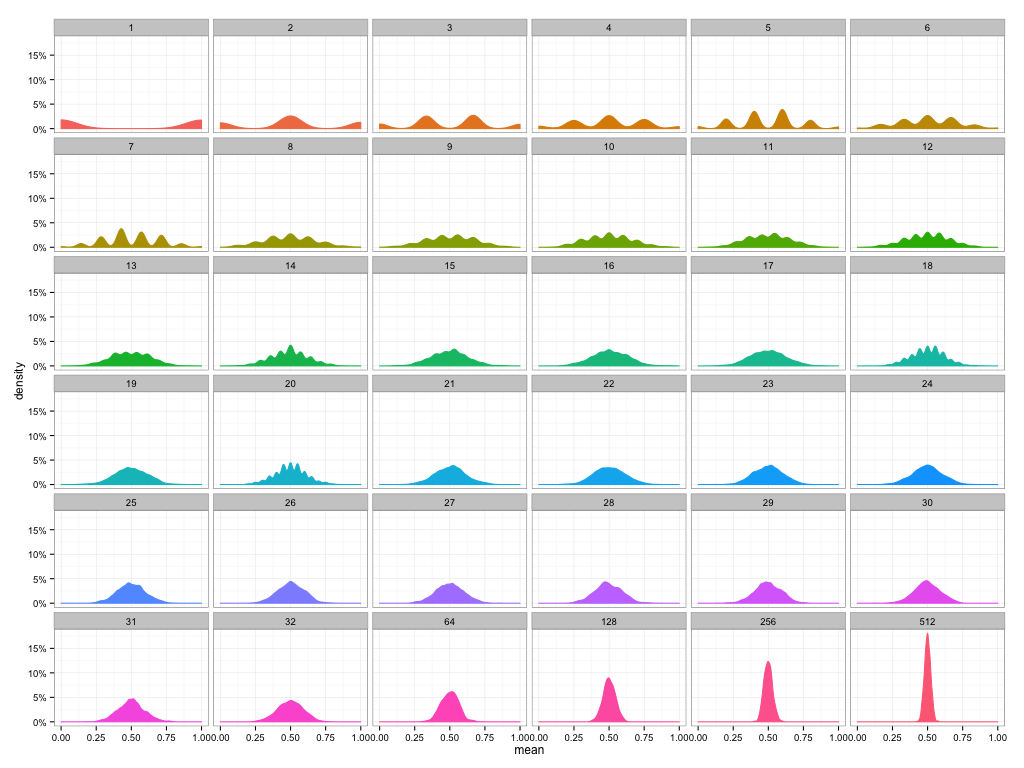
\includegraphics[width=0.9\textwidth]{img/6-central-limit-theorem.png}
    \caption{A simulation using the binomial distribution. Random 0s and 1s were generated, and then their means calculated for sample sizes ranging from 1 to 512. Note that as the sample size increases the tails become thinner and the distribution becomes more concentrated around the mean.(From Wikipedia.org)}
    \label{fig:6-1}
\end{figure}

\subsection{Other Applications of the Central Limit Theorem}

\begin{proposition}
    Let $X_1,\dots,X_n$ be a random sample from a distribution for which only positive values are possible($P(X_i > 0) = 1$). Then if $n$ is sufficiently large, the product $Y=X_1X_2\cdot\cdots\cdot X_n$ ahs approximately a lognormal distribution; that is, $\ln(Y)$ has a normal distribution.
\end{proposition}

\subsection{The Law of Large Number}